\documentclass[a4paper, 10pt]{article}
\usepackage[margin=1in]{geometry} 
\usepackage{amsmath}
\usepackage{tcolorbox}
\usepackage{amssymb}
\usepackage{amsthm}
\usepackage{lastpage}
\usepackage{fancyhdr}
\usepackage{accents}
\usepackage{titlesec}
\usepackage{graphicx}
\usepackage{hyperref}

\usepackage{titling}
\usepackage[export]{adjustbox}

\usepackage{enumitem}
\setlist{nolistsep}

\usepackage[scaled]{helvet}
\renewcommand\familydefault{\sfdefault} 
\usepackage[T1]{fontenc}
\usepackage{tcolorbox}
\definecolor{light-blue}{cmyk}{0.24, 0.12, 0.0, 0.04, 1.00}

\setlength{\parindent}{0pt}
\setlength{\parskip}{6pt}%

%parskip shold take care of heading spacing
\titlespacing\section{0pt}{0pt}{0pt}
\titlespacing\subsection{0pt}{0pt}{0pt}
\titlespacing\subsubsection{0pt}{0pt}{0pt}


\pagestyle{fancy}
\setlength{\headheight}{40pt}

\hypersetup{
    colorlinks=true,
    linkcolor=blue,
    filecolor=magenta,      
    urlcolor=black,
    pdfpagemode=FullScreen,
}

\begin{document}

%REPLACE THE TEXT BELOW WITH YOUR NAME, STUDENT NUMBER AND ASSIGNMENT NUMBER
\lhead{Alexander Sepelenco (20335014)} 
\rhead{CS7GV6 – Computer Graphics Deliverable 2} 
\cfoot{\thepage\ of \pageref{LastPage}}

\begin{tcolorbox}[colback=light-blue]
\begin{small}
\textbf{DECLARATION:} I understand that this is an \textbf{individual} assessment and that collaboration is not permitted. I have read, understand and agree to abide by the plagiarism provisions in the
General Regulations of the University Calendar for the
current year, found at http://www.tcd.ie/calendar.
I understand that by returning this declaration with my work, I am agreeing with the above statement. 
\end{small}
\end{tcolorbox}

\bigskip
%OPTIONAL: INSERT A TITLE BY UN-COMMENTING THE NEXT LINE
%\Large\textbf{Project Proposal and Design Document} \normalsize

%15/10/2024: Deliverable 1 - Project Proposal and Design Document (5 Marks)
%    Submit a written proposal (1-2 pages) outlining your intended underwater ecosystem
%    Describe key features you plan to implement (types of marine life, lighting effects, unique interactions)
%    Mention any advanced or custom features that you are considering
%    Include sketches, diagrams or screenshot illustrating the scene layout


% a short pdf report with clear code snippets showing your implementation of the hierarchy, 
% and camera control, with clear comments.



% Basic Scene Setup and Object Loading (15 Marks): Based on your selected theme, create a cohesive 3D underwater environment with water including 3D models, and terrain.
% User Camera Control (10 Marks): Implement user camera movement for scene exploration. Basic controls (e.g., forward, backward, left, right) are required, 
%   with additional marks for more complex camera interactions.
% Hierarchical Animation (10 Marks): Animate at least one creature or object with a hierarchical structure (e.g., a fish with fins, plants swaying). 
%   Marks are awarded based on the hierarchy's meaningful use and complexity.

\section{Implementations}
This section will discuss my implementations of hierarchy, camera controls, and other relevant aspects for this deliverable.
The reiterate my project title is: 
"Manta Ray Migration - Simulate a large school of manta rays gliding through a dynamic ocean, interacting with smaller fish".

\subsection{Basic, Scene Setup and Object Loading}
In my scene there are Manta Rays, small fish, starfish, seaweed, and textured environments with movements using Boids \cite{boids}.
The video attached to the deliverable shows a video demonstration of the scene loading and running. The written explanation, is
I have functions which wrap opengl calls, in object\_create, object\_draw, and object\_destroy, which have a dependency on shaders.
Shaders are attached during initialisation at the beginning and in a loop is drawn with the models. In certain cases, a generic model
structure is not used, and instead structures like "Mantaray", and "Fish", exist which in practice extends the functionality of what 
a model is. Below is an example of my Model struct followed by Mantaray struct:

\begin{figure}[h]
    \centering
    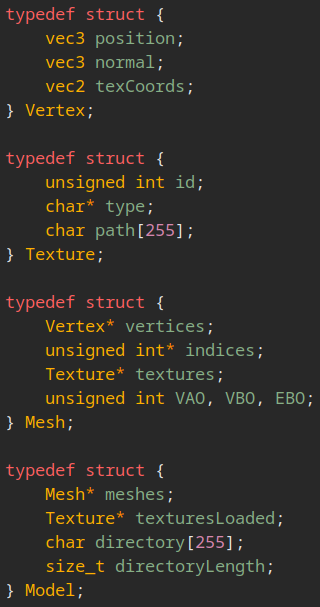
\includegraphics[scale=1.0]{images/model-struct}
    \caption{Structure definition of Model}
    \label{fig:model-struct}
\end{figure}

\newpage

\begin{figure}[h]
    \centering
    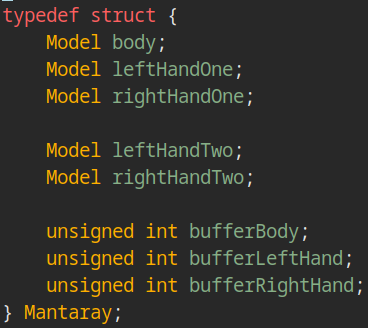
\includegraphics[scale=1.0]{images/mantaray-struct}
    \caption{Structure definition of Manta Ray}
    \label{fig:mantaray-struct}
\end{figure}

My Model struct is based of the material I referenecd for model loading from LearnOpenGL, \cite{learnopengl}.
My Manta Ray struct is defined in a specific way to allow for hierarchical animation. I split the model into multiple parts.
I also create multiple buffers, to draw these models using instancing, a way of drawing multiple equivalent objects in one
draw call. 

\subsection{Camera}
My camera's implementation is based on euler angles, where, yaw, pitch, are used. Notice how roll isn't used, the camera wouldn't
need to roll as I am mimicking a first person perspective. I have a mouse field which I set as well to move the camera.
The structure definition of the camera can be seen below:
An important part of my camera implementation, is that I had additional structure, called "Cameras". This allows me to pass in multiple
Camera structures and in turn give my code the ability to change cameras with a click of a button. Additionally zoom functionlity exists,
which increases and decreases the field of view using perspective. 

\begin{figure}[h]
    \centering
    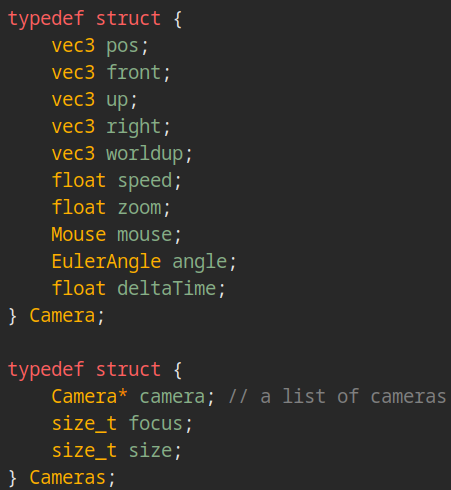
\includegraphics[scale=0.8]{images/camera-struct}
    \caption{Structure definition of Camera and Cameras}
    \label{fig:camera-struct}
\end{figure}

\begin{figure}[h]
    \centering
    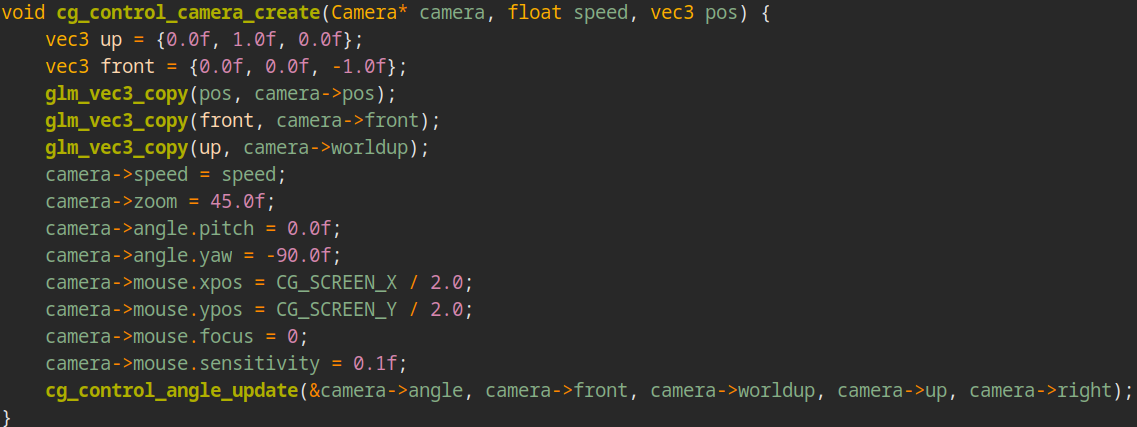
\includegraphics[scale=0.5]{images/camera-create-2}
    \caption{Creation of Camera}
    \label{fig:camera-create-2}
\end{figure}

\begin{figure}[h]
    \centering
    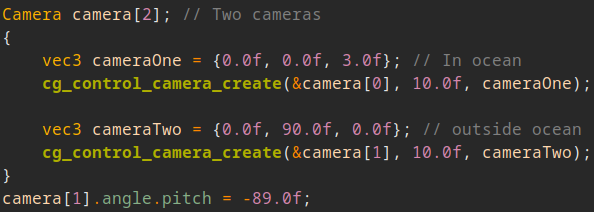
\includegraphics[scale=0.9]{images/camera-create}
    \caption{Structure initialisation of camera}
    \label{fig:camera-create-2}
\end{figure}

\newpage

\begin{figure}[h]
    \centering
    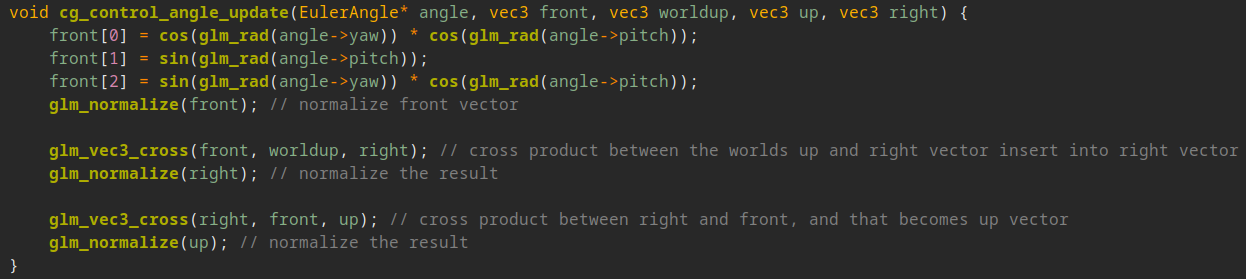
\includegraphics[scale=0.6]{images/camera-update}
    \caption{Structure initialisation of camera}
    \label{fig:camera-create-2}
\end{figure}

\begin{figure}[h]
    \centering
    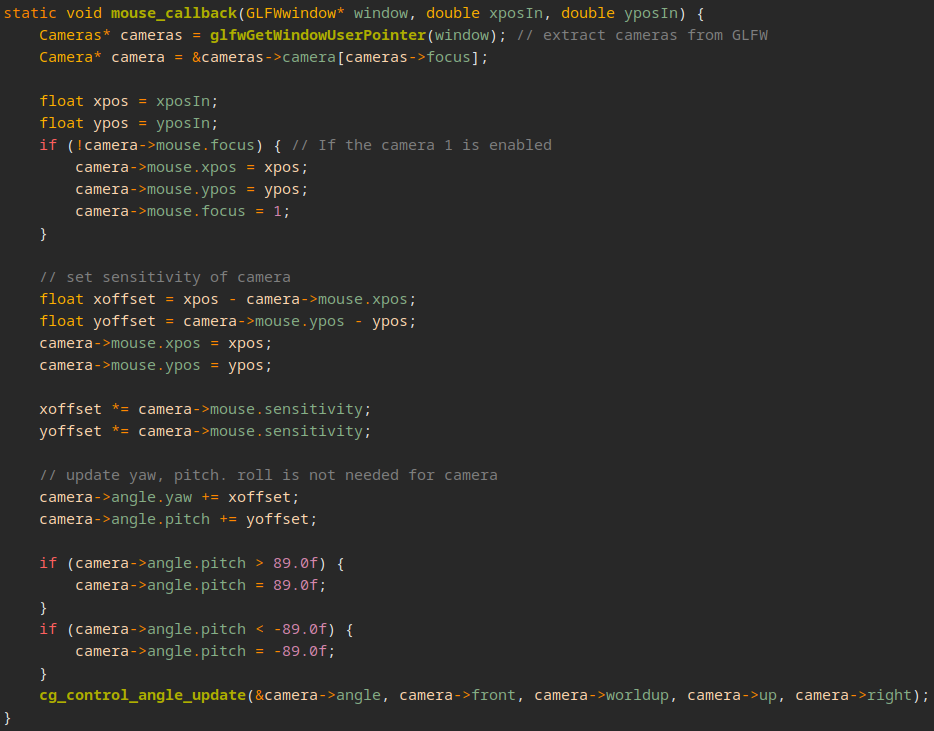
\includegraphics[scale=0.8]{images/camera-mouse}
    \caption{Mouse movement for camera}
    \label{fig:camera-create-2}
\end{figure}

\newpage

Camera switching is achieved by calling a GLFW function. This function allows the user to pass in a pointer to a GLFW window, this window
will hold the cameras structure, and anywhere in the code where I pass my window, I can extract the cameras and modify the camera. This is important
when we update the camera at each iteration of the render loop. I have a focus variable which determines
which camera is on. Therefore in practice I have two cameras which I can switch, and the angles of the cameras stay consistent when rapidly switching.
My cameras are set to be inside the "ocean", and outside, looking at the skybox.

\newpage
\subsection{Hierarchical Animation}
Two of my models use hierarchical animation, the Manta Ray and the small fish. I will use Manta Ray as the example for my explanation.
My Manta Ray, is split into separate models, this is to ensure I can rotate, and therefore animate the fish. The models are split into:
left hand 1, left hand 2, body, right hand 1, right hand 2. I use hands as a generic term to refer to what makes them flapping motion. It is split
into two, which I animate in a hiearchical way. My "left/right hand 1" rely on "body", I do this by multiplying the "left/right hand 1" by "body". I do the same
for "left/right hand 2" which multiplies by "left/right hand 1". Below is a code snippet which I have also commented. It goes through the hierarchical animation
and the movement of the mantaray for it's left hands. The same approach is used for the right hands, but it is not shown here for the sake of brevity.

\begin{figure}[h]
    \centering
    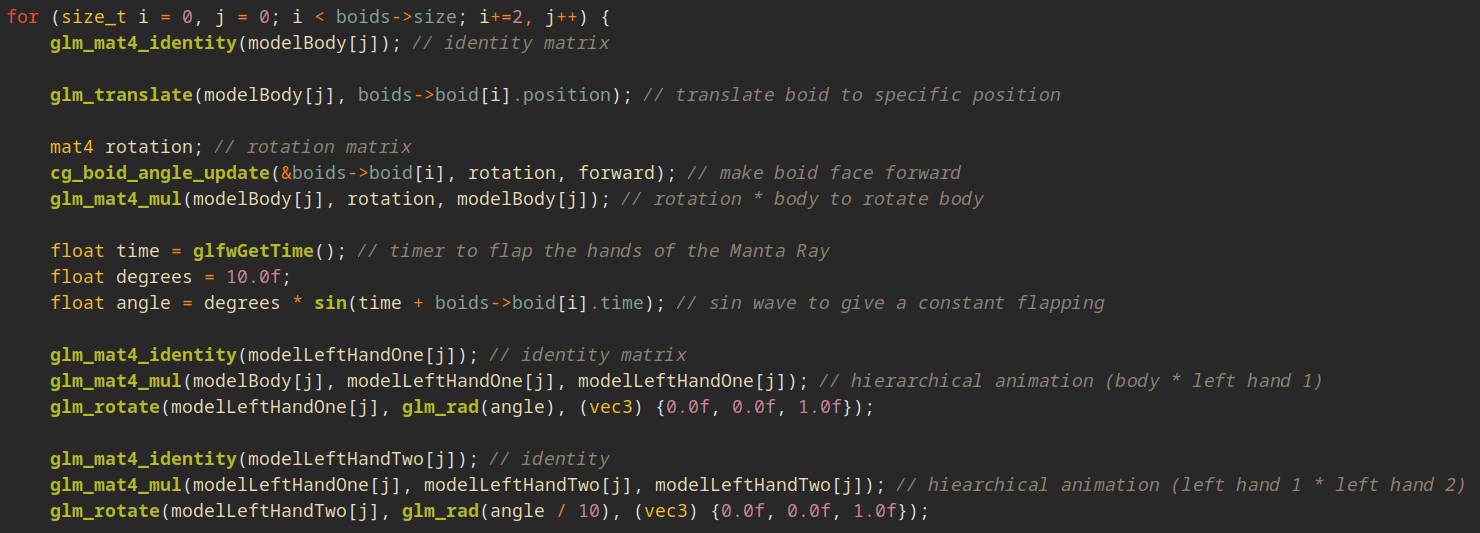
\includegraphics[scale=0.5]{images/mantaray-hanim}
    \caption{Mantaray Hierarchical animation Code}
    \label{fig:mantaray-animation}
\end{figure}

\begin{figure}[h]
    \centering
    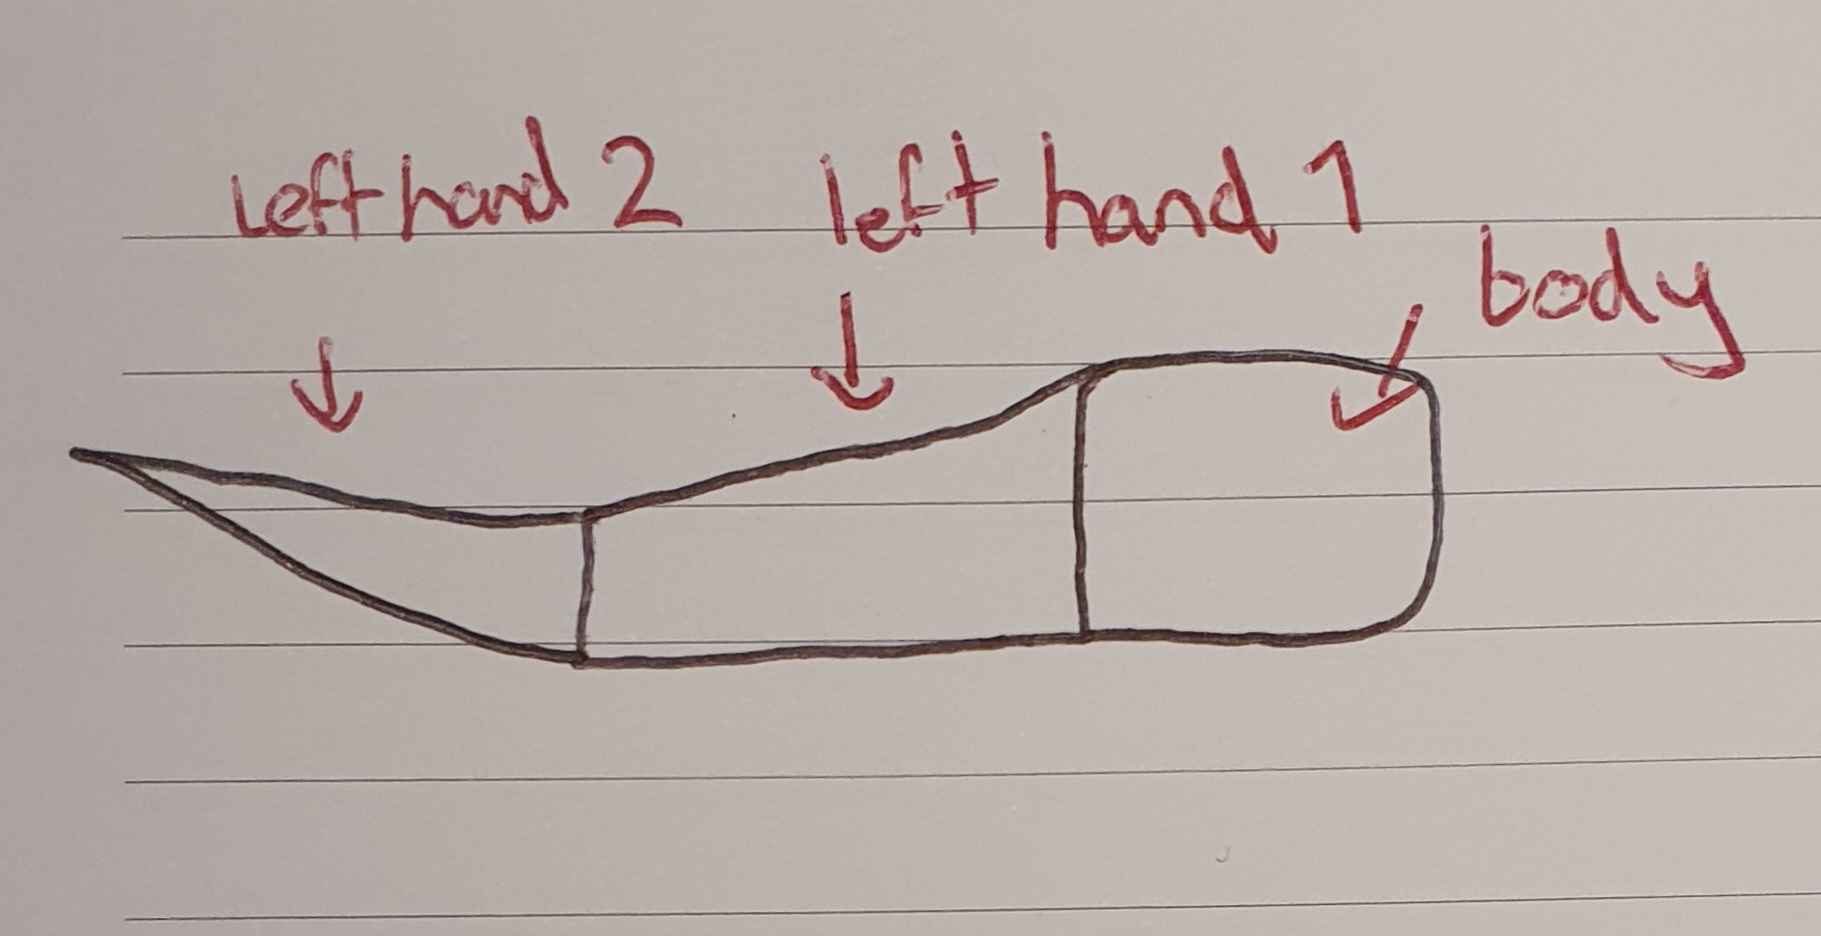
\includegraphics[scale=0.2]{images/mantaray-anim}
    \caption{Mantaray Hierarchical structure}
    \label{fig:mantaray-animation}
\end{figure}

\subsubsection{Other Animation aspects}
Animations outside of hierarchical were also used. Quaternions using builtin cglm linear algebra functions
\cite{cglm}, were used to rotate my models. My Models "swim" based on the boids algorithm \cite{boids}. 
Whenever a wall is hit, the Manta Ray and small fish would rotate. I used SLERP, to spherically linearly 
interpolate the positions and give a smooth rotation of my models. I use a lot of the builtin cglm functions 
given to me to achieve this. A visual demonstration might make sense, so reference the video for how the animation
behaves.

\begin{figure}[h]
    \centering
    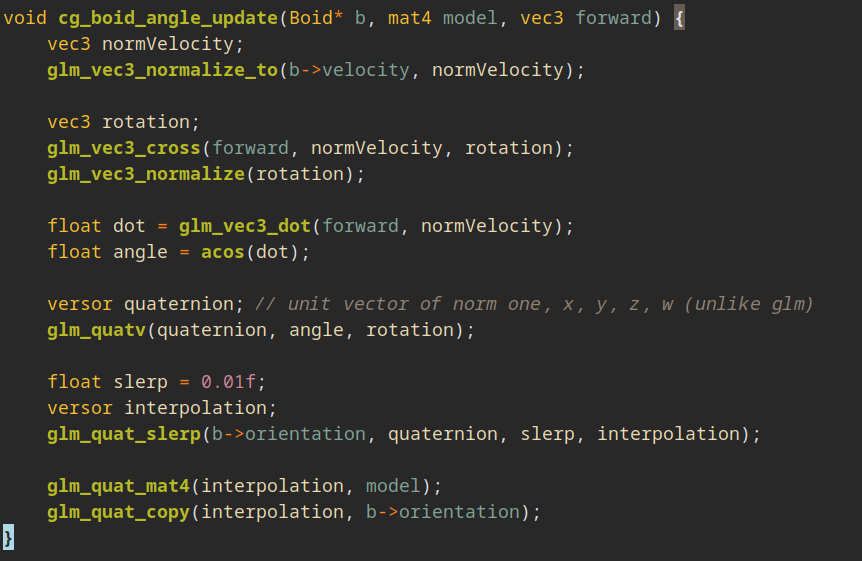
\includegraphics[scale=0.8]{images/boids-lerp}
    \caption{Spherical lerp animation}
    \label{fig:mantaray-animation}
\end{figure}

\newpage

\begin{thebibliography}{9}
\bibitem{boids}
Boids: Artifical life Simulation
\textit{https://en.wikipedia.org/wiki/Craig\_Reynolds\_(computer\_graphics)}
\textit{Craig Reynolds}

\bibitem{learnopengl}
LearnOpenGL: Modern Opengl references
\textit{https://learnopengl.com/}
\textit{JoeyDeVris}

\bibitem{cglm}
cglm: an optimized 3D math library written in C99 (compatible with C89). 
It is similar to the original glm library, except cglm is mainly for C.
\textit{https://cglm.readthedocs.io/en/latest/}
\textit{recp}
\end{thebibliography}


\end{document}


